\section{A Top-Down Approach to Low-Energy Phenomenology: mSUGRA}

\begin{frame}{The mSUGRA Framework I}
\addtocounter{framenumber}{-1}
\begin{figure}
	\centering
	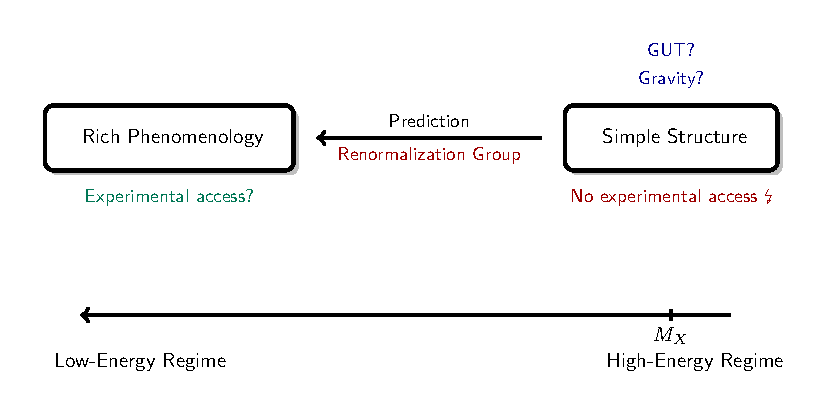
\includegraphics[scale = 1]{figures/mSUGRA_idea}
\end{figure}
\end{frame}

\begin{frame}{The mSUGRA framework II}
\begin{itemize}
	\item Want to naturally include \alert{gravity}, or more precisely \alert {local SUGRA}.\\[1em]
	\item SUGRA is broken at some high energy scale, usually at around $M_{\mathrm{Planck}}\sim 10^{19}\ \mathrm{GeV}$.\\[1em]
	\item Assume \alert{gravity-mediated SUSY breaking}, i.\,e. $m_{\mathrm{soft}} \sim \frac{\langle F\rangle}{M_{\mathrm{Planck}}}$\\[1em]
\end{itemize}
The general idea is now to assume a \alert{\enquote{minimal} normalization} of the kinetic terms in the SUGRA Lagrangian, i.\,e.
\begin{equation*}
	\mathcal{L}_{\mathrm{SUGRA}} \supset-\frac{1}{M_{\mathrm{Planck}}} F\left(\frac{1}{2} \ \alert{\alpha}\ \lambda \lambda+\frac{1}{6} \ \alert{\beta}\  \phi \phi \phi+\frac{1}{2} \ \alert{\gamma}\ \phi \phi\right)+\mathrm{h.c.}-\frac{1}{M_{\mathrm{Planck}}^{2}} F F^{*} \ \alert{\delta}\ \phi \phi^*
\end{equation*}\\[0.5em]

Comparison with initial $\mathcal{L}_{\mathrm{soft}}$ $\implies$ Simple relations for the input parameters!
\end{frame}

\begin{frame}{Finding the correct initial Conditions}	
The relatively simple form of the kinetic terms allows to simplify the structure of the relevant couplings at the initial scale as follows:\\[1em]
	\begin{itemize}
		\item scalar squared-masses are \alert{flavor-diagonal} and \alert{universal}: 
	\end{itemize}
	\begin{align*}
				m^2_{\tilde{q}}(M_X) &= 	m^2_{\tilde{u}}(M_X) = m^2_{\tilde{d}}(M_X) = m_0^2 \mathbb{1} \\[0.5em]
				m^2_{\tilde{\ell}}(M_X) &= 	m^2_{\tilde{e}}(M_X) = m_0^2 \mathbb{1} \\[0.5em]
				m^2_{1}(M_X) &= 	m^2_{2}(M_X) = m_0^2 
	\end{align*}
		\begin{itemize}
		\item the same is true for the $A$-parameters:
	\end{itemize}
	\begin{align*}
				A^{U} (M_X) = A^{D} (M_X) = A^{E} (M_X) = A_0^2 \mathbb{1}
	\end{align*}
	\begin{itemize}
		\item Additionally we assume unification of the (tree level) gaugino masses:\\[1em]
		
		\end{itemize}
	 \begin{align*}
				M_1 (M_X) = M_2 (M_X) = M_3 (M_X) = m_{1/2} 
	\end{align*}
	\end{frame}

\begin{frame}{Renormalization Group Equations}
This allows us to compute the low-energy MSSM parameters with the help of standard \alert{renormalization group techniques}!\\[1em]

	\textbf{Reminder:} The \alert{beta function} $\beta(g)  = \frac{\partial g}{\partial \operatorname{ln} M}$ is the rate of change of the renormalized coupling at\\[0.3em] the scale $M$, where the bare coupling is fixed \cite{PeskinSchroeder1995}.\\[1em]
	For example, we get the following result for the low-energy gaugino mass parameters:
	\begin{equation*}
		M_{i}=\frac{\alpha_{i}\left(M_{Z}\right)}{\alpha_{\mathrm{GUT}}} m_{1 / 2} \longrightarrow M_{3}\left(M_{Z}\right)=\frac{\alpha_{3}\left(M_{Z}\right)}{\alpha_{2}\left(M_{Z}\right)} M_{2}\left(M_{Z}\right)=\frac{\alpha_{3}\left(M_{Z}\right)}{\alpha_{1}\left(M_{Z}\right)} M_{1}\left(M_{Z}\right)
	\end{equation*}
	This results in the well known relation: 
	\begin{equation*}
		M_{1}=\frac{5}{3} \operatorname{tan}^{2} \theta_{W} M_{2} \sim \frac{1}{2} M_{2}
	\end{equation*}
	\end{frame}

\begin{frame}{Solution of the RGEs for mSUGRA}
	\begin{figure}
	\centering
	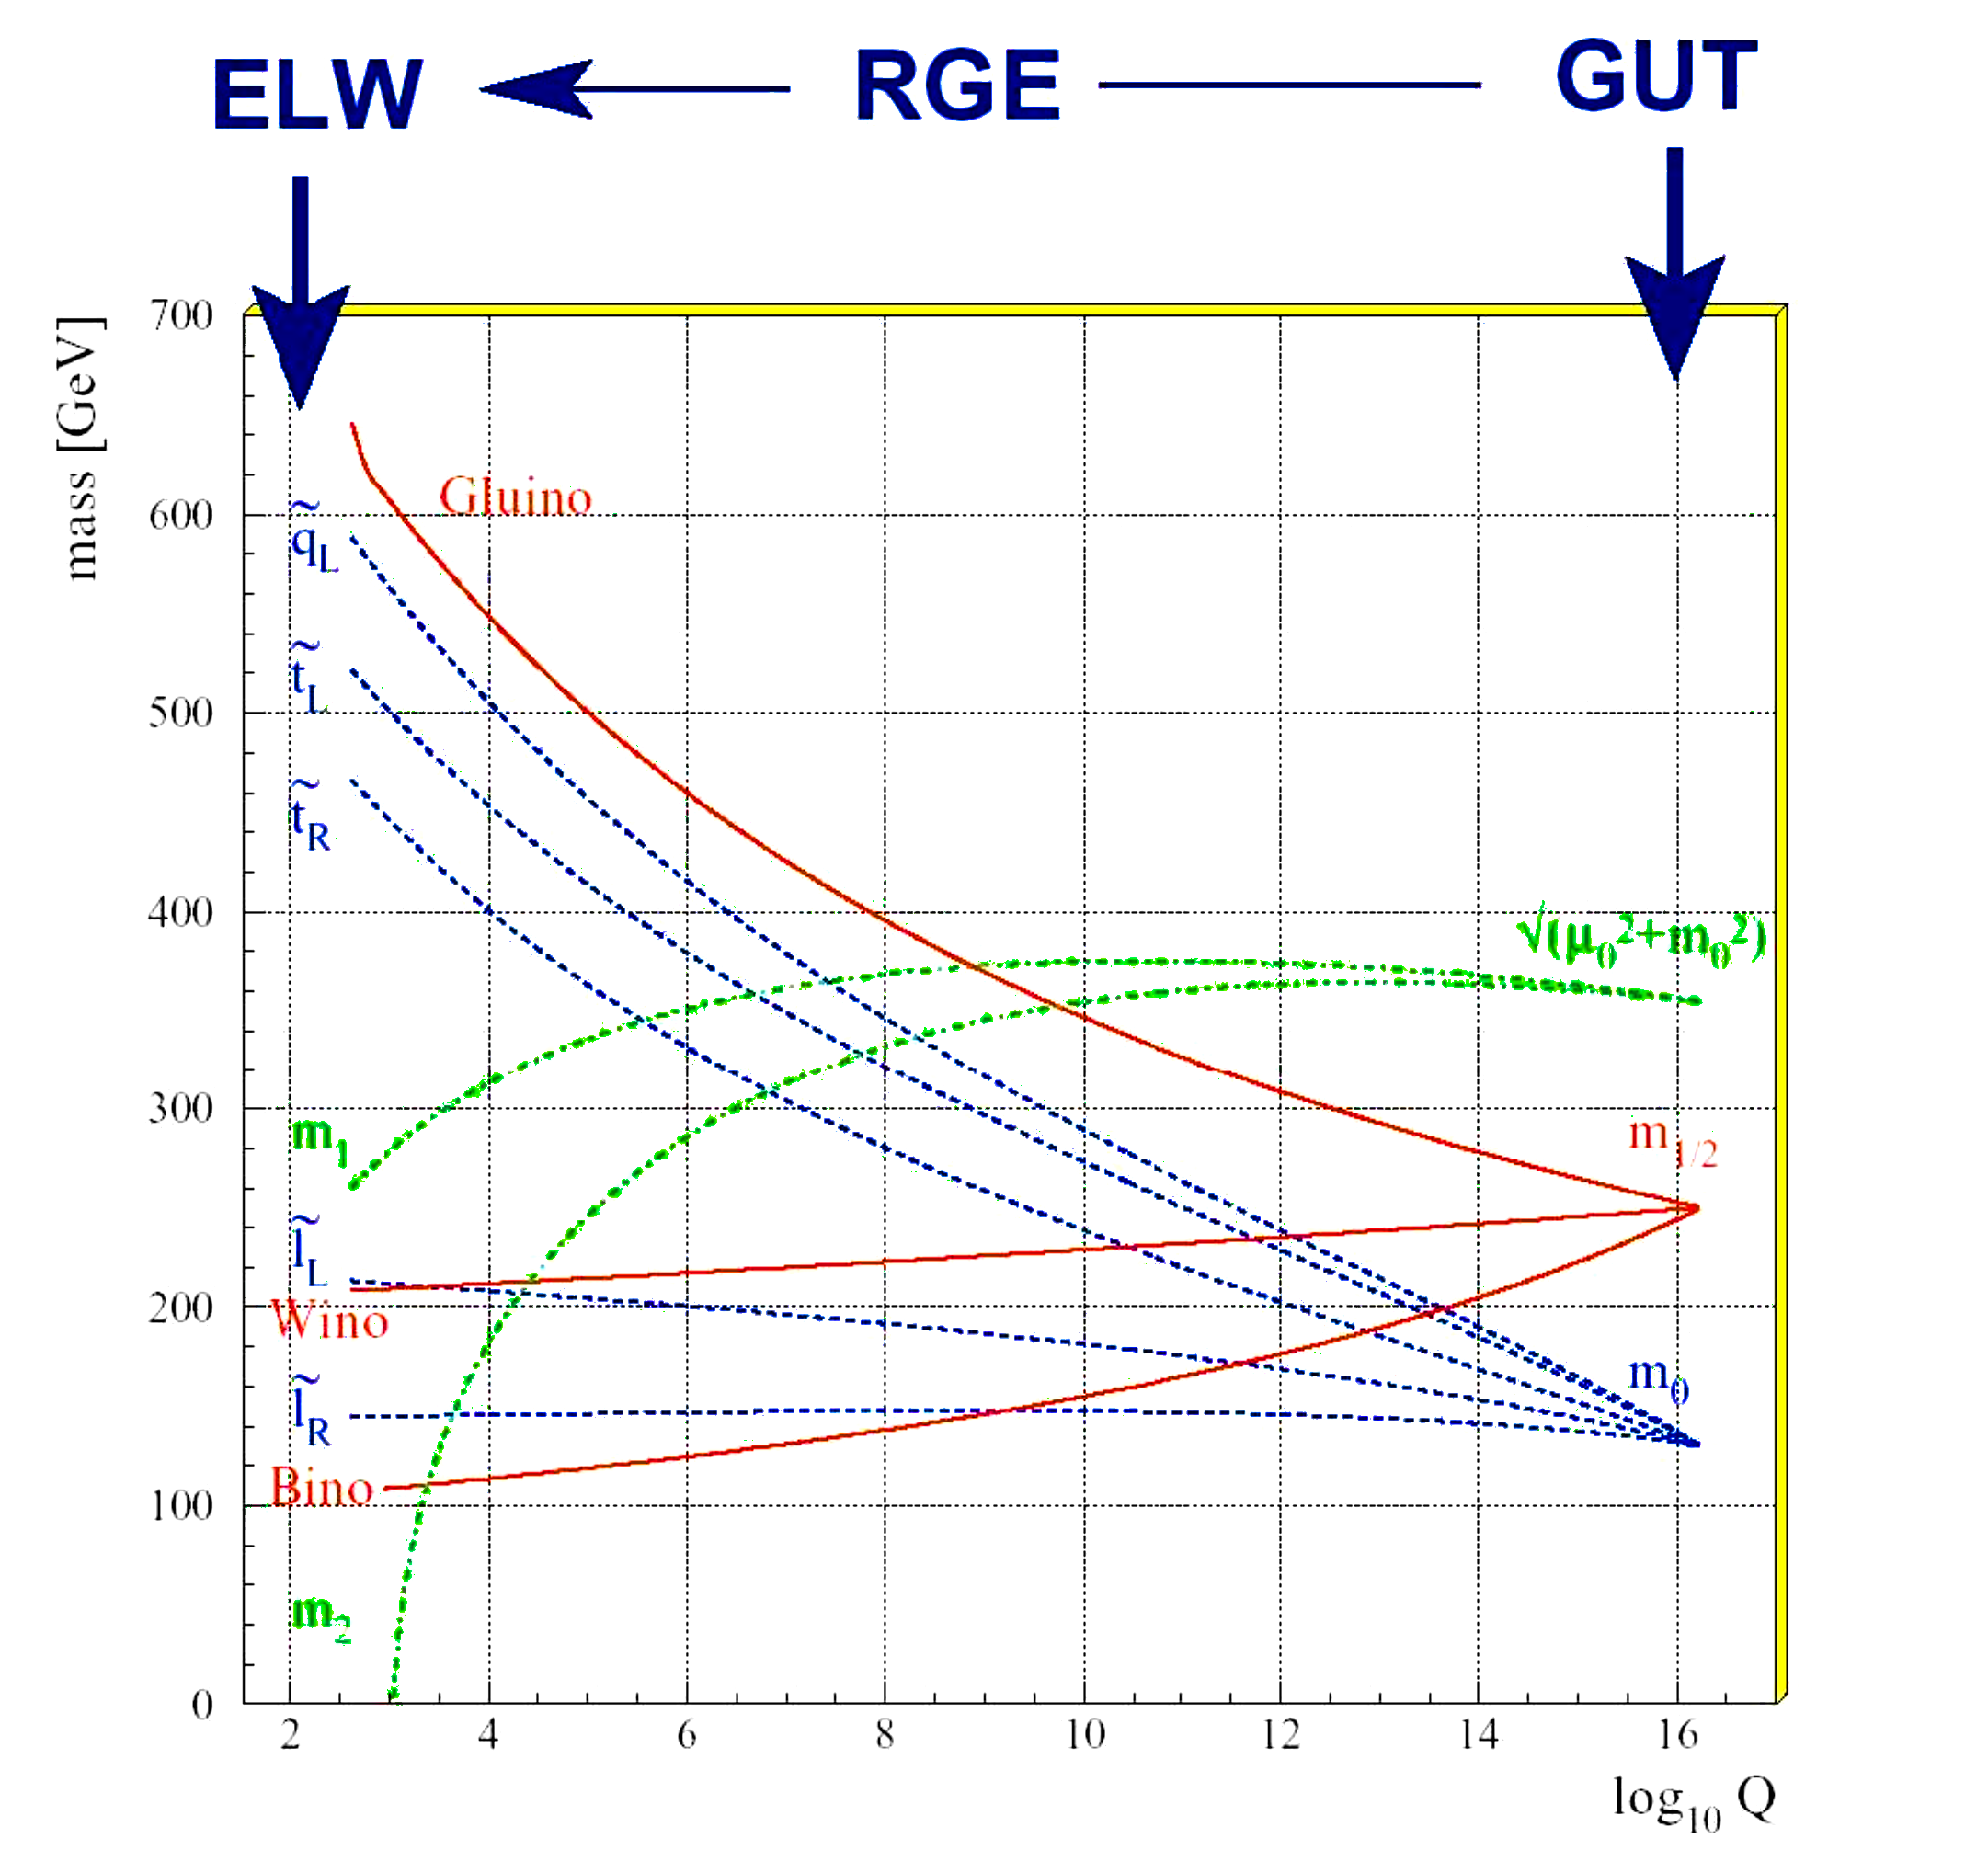
\includegraphics[scale = 0.75]{figures/mSUGRA_RGE}
	\caption{Running of the mSUGRA parameters\footnote{Figure taken from: \tiny\url{https://www.physi.uni-heidelberg.de/~uwer/lectures/ParticlePhysics/Vorlesung/Lect-10b.pdf} (10.02.21)}.}
	\end{figure}
\end{frame}
\begin{frame}{Parameter Count in the mSUGRA Framework}
This means in total we are left with only the following \alert{four continuous} and \alert{one discrete} free parameters in the mSUGRA model:\\[1em]

\begin{itemize}
	\item $\tan\beta$, the ratio of the VEVs in the two-Higgs doublet model\\[1em]
	\item $m_{1/2}$, the universal gaugino mass\\[1em]
	\item $m_{0}$, the universal scalar (sfermion/Higgs) mass\\[1em]
	\item $A_{0}$, the universal trilinear coupling\\[1em]
	\item $\operatorname{sign}(\mu)$, the sign of the Higgs-higgsino mass parameter\\[1em]
\end{itemize}
The relations for $\tan\beta$ and $\abs{\mu}$ come from the \alert{two minimum conditions} for the Higgs potential.\\[1em]
\textbf{Remark:} Additional requirements such as the unification of the top, bottom and tau Yukawa couplings at the GUT scale further restricts the possible values of $\tan\beta$ and $A_0$.
\end{frame}

\begin{frame}{Map of the mSUGRA Parameter Space}
	\begin{figure}
	\centering
	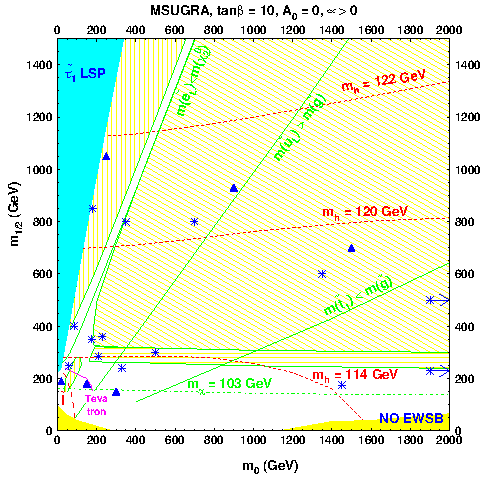
\includegraphics[scale = 0.85]{figures/parameter_space_mod}
	\caption{Map of the mSUGRA parameter space for different values of the universal mass parameters, \\ slightly adapted from \cite{CMS2007}.}
	\end{figure}
\end{frame}